\subsection{Zusammenfassung}

\begin{frame}
	\frametitle{Zusammenfassung}
	\begin{itemize}
		\item Klima ist der mittlere Zustand der Atmosphäre an einem bestimmten Ort über einen längeren Zeitraum
		\item Atmosphäre und Strahlungshaushalt der Erde erzeugen lebensfreundliche Bedingungen auf der Erde
		\item Der natürliche Treibhauseffekt entsteht vorallem durch Wasserdampf und CO$_2$.
		\item CO$_2$, CH$_4$ und N$_2$O sind starke Treibhausgase
		\item Durch den Anstieg der atmosphärischen Konzentrationen dieser drei seit der Industrialisierung kann der Mensch als Ursache angenommen werden.
		\item Die Komponenten des Klimasystems hängen stark zusammen, sodass Veränderungen eines Faktors zum Teil deutliche Folgen in anderen Bereichen erzeugen kann.
		\item Manche Änderungen treten erst nach hunderten Jahren auf, manche sind aber auch schon heute und in wenigen Jahren spürbar!
	\end{itemize}
\end{frame}

\begin{frame}
	\frametitle{Zusammenfassung und Ausblick}
	\begin{figure}
		\centering
		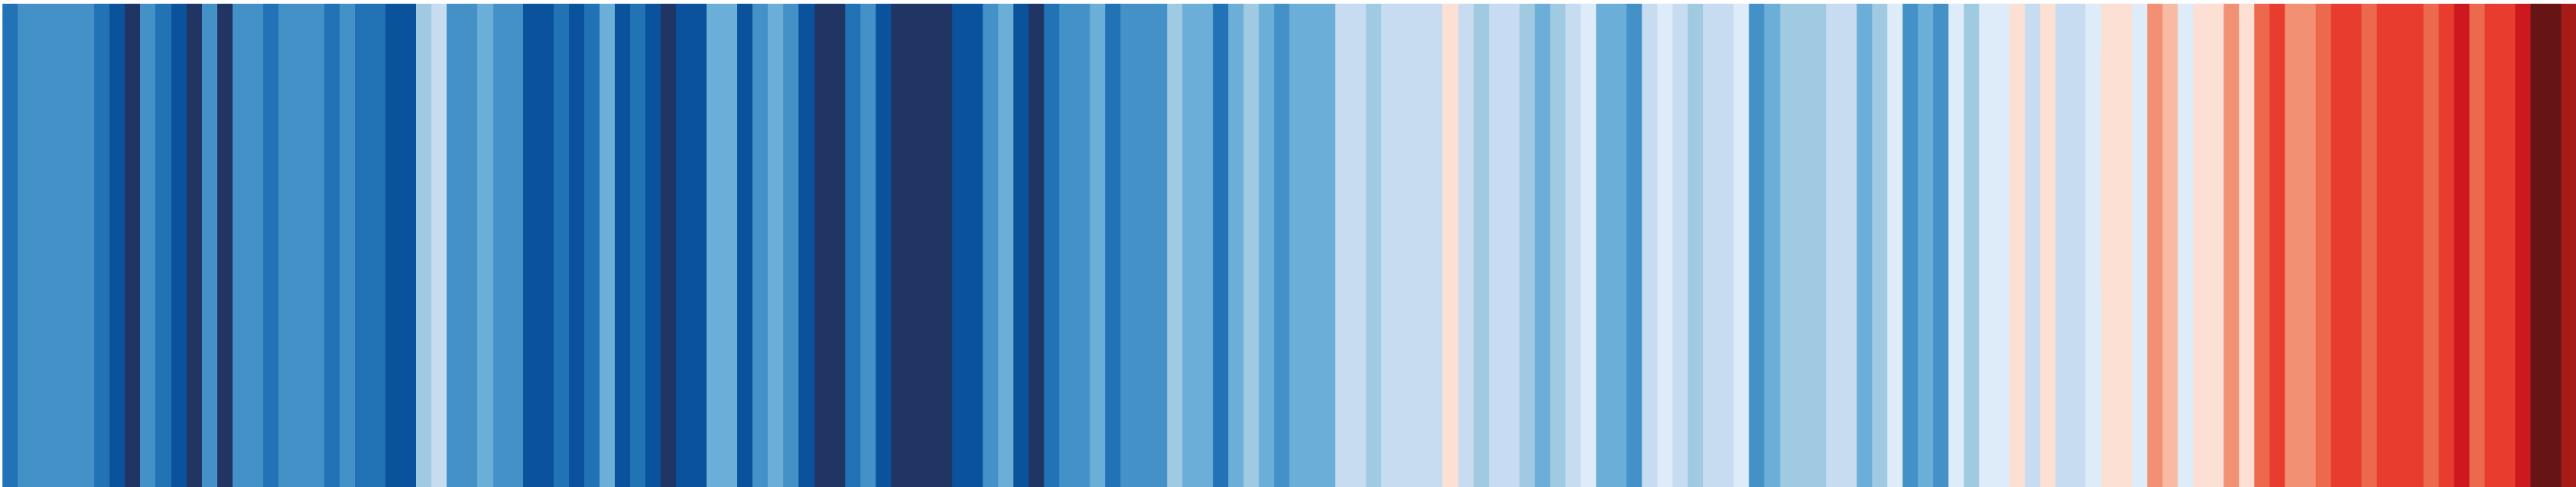
\includegraphics[width=\linewidth]{bilder/s4f-warming-stripes}
		\caption{Die Warming Stripes}
	\end{figure}
	$\rightarrow$ Die langfristige Erwärmung und Häufung extremer Wetterereignisse bedeutet eine Veränderung des Klimas!\\
	$\rightarrow$ Viele dieser Änderungen sind in Modellen der Klimaforscher relativ genau vorherzusagen. \\
	$\rightarrow$ Das Ausmaß einiger Änderungen sind aufgrund der langfristigen Effekte nicht konkret vorherzusagen, aber die Tendenz ist klar.
\end{frame}
